\chapter{Avaliação} \label{chp:LABEL_CHP_5}

Neste capítulo apresentamos as avaliações que foram realizadas a partir dos algoritmos implementados. Na primeira etapa, avaliamos o desempenho da máquina de vetores suporte a partir da porcentagem de acertos da classificação. Na segunda etapa avaliamos o desempenho da paralelização do nosso programa. 
Para isso, medimos o tempo de execução da aplicação e o {\em speedup} (aceleração) obtido com a versão paralela.

Todos os experimentos foram realizados no sistema operacional Windows 10, em uma máquina com CPU Intel Core i7-4770 @ 3.4GHz. A GPU utilizada foi uma NVIDIA GeForce GTX 660 com 1152 Cores e 1.58GB de memória.

\section{Conjuntos de Dados}\label{sec:LABEL_CHP_5_SEC_A}
Para avaliar as aplicações desenvolvidas, selecionamos três conjuntos de dados, denominados  {\em Iris}, {\em Adult} e {\em Web}, os quais podem ser encontrados no site do repositório de dados da UCI \cite{UCI} e no site do LIBSVM \cite{art:LIBSVM}. O conjunto {\em Iris} foi selecionado por ser pequeno e linearmente separável, os conjuntos \emph{Adult} e \emph{Web} foram selecionados entre os conjuntos usados por \cite{art:REF_ART_1} e \cite{art:REF_ART_2} por terem muitos exemplos no conjunto de dados e por serem binários (só possuem duas classes).

\subsection{Iris} \label{sec:Iris}
Esse conjunto de dados distingue 3 tipos de iris, uma especie de flor. Os atributos descrevem os tamanhos das pétalas e das sépalas. Cada exemplo possui 4 atributos. São 150 exemplos no conjunto.
\subsection{Adult} \label{sec:Adult}
O objetivo desse conjunto de dados é analisar a faixa de renda de um adulto americano baseado em diversos fatores. A classificação prevê se o individuo tem renda de mais ou menos que 50 mil dólares por ano. Alguns dos atributos são idade, país de origem, etnia, estado civil e escolaridade. Cada exemplo possui 119 atributos. Existem 9 versões desse conjunto de dados variando o número de amostras entre 1605 e 16100.
\subsection{Web} \label{sec:Web}
Esse conjunto de dados determina se uma página pertence a uma categoria ou não baseado na presença de palavras chave. Cada exemplo possui 300 atributos que representam se uma palavra esta presente ou não na página. Existem 8 versões desse conjunto de dados variando o número de amostras entre 2477 e 17188.

\subsection{Tratamento dos dados}
No conjunto {\em Iris}, foi necessário remover uma das classes para que o conjunto fosse compatível com o classificador binário. As duas classes remanescentes são linearmente separáveis de forma que o conjunto serviu para facilitar os testes no início do desenvolvimento.

O conjunto \emph{Adult} possui atributos simbólicos não-binários, com valores possíveis definidos em conjuntos finitos, como por exemplo $PaisDeOrigem \in \left [ Brasil,Espanha,Noruega \right ]$. É preciso atribuir valores numéricos para esses atributos para que funcionem com a máquina de vetores suporte. Para isso trocamos cada um desses atributos por atributos binários. Substitui-se o atributo $PaisDeOrigem$, por 3 atributos binários que podem ser verdadeiro ou falso, $Brasileiro \in \left [ 0,1 \right ]$, $Espanhol \in \left [ 0,1 \right ]$ e $Noruegues \in \left [ 0,1 \right ]$. Os conjuntos de dados disponíveis no site do LIBSVM já foram convertidos para esse padrão. O conjunto \emph{Adult} possuía 14 atributos multivariados que foram convertidos em 119 atributos binários.

\section{Métricas de avaliação}
Para avaliar nossa máquina de vetores suporte, medimos a porcentagem de acertos de nosso programa. Para isso, calculamos a porcentagem de casos de teste que conseguimos classificar corretamente durante a validação cruzada. 
%[REF] Dietterich, T.G., 1997. Approximate statistical tests for comparing supervised classification learning algorithms. Neural Computation, vol. 10, pp. 1895–1924.
%Usando validação cruzada, para construir cada par de conjuntos de treinamento e de teste, o conjunto de dados é dividido aleatoriamente em n conjuntos disjuntos de igual tamanho (chamados partições), T1, ..., Tn. Então são conduzidas n rodadas. Em cada rodada, o conjunto de teste é Ti e o conjunto de treinamento é a união de todos os outros Tj, j diferente de i. A precisão então é dada pela média das porcentagens de acertos das n rodadas.


Para avaliar nossa paralelização, comparamos o tempo de execução sequencial e paralelo com conjuntos de teste de tamanhos diferentes. O tempo medido foi o tempo total de execução do programa. Escolhemos não comparar somente o tempo de treinamento ou classificação pois isso não levaria em consideração o tempo em que se copia dados para a memória da GPU. A partir dos tempos medidos, calculamos o speedup (ou aceleração), que é uma métrica de avaliação comum de paralelização onde se divide o tempo sequencial pelo paralelo, $\frac{t_{sequencial}}{t_{paralelo}}$. 
%silvana: quais parâmetros são esses???
%Para que essa fosse uma comparação justa, todos os parâmetros foram iguais para versão sequencial e paralela. 
%Felipe: Mudei isso para a próxima sessão
Para essa avaliação utilizamos os conjuntos \emph{Web} e \emph{Adult} com diferentes tamanhos.

\section{Avaliação da Máquina de Vetores Suporte}
Avaliamos nossa implementação do algoritmo Kernel-Adatron definindo, primeiramente, quais parâmetros nos dão um bom resultado em porcentagem de acerto. Para isso, fizemos uma série de testes com conjuntos de dados pequenos e uma validação cruzada de poucas partições.

Para fazer essa análise permutamos todos os parâmetros da tabela \ref{tab:testParameters1}, ou seja, experimentamos cada uma das combinações possíveis entre os valores da tabela, com exceção dos parâmetros marcados com *, que só afetam a versão sequencial ou só afetam a versão paralela.

\begin{table}
    \caption{Parâmetros Usados na Primeira Rodada de Testes}
    \label{tab:testParameters1}
    \centering
    \begin{tabular}{|c|c|} \hline
        Parâmetro & Valores Utilizados \\ \hline
        -sd & 0 \\ \hline
        -f & 3 \\ \hline
        -mi & 512 \\ \hline
        -l & r \\ \hline
        -p & 1e-2, 1e-4, 1e-8 \\ \hline
        -st & 1, 1e-1, 1e-2, 1e-3 \\ \hline
        -sm & s, m \\ \hline
        -d & a1, w1\\ \hline
        -svm & p, s\\ \hline
        -t* & 32, 128, 512\\ \hline
        -ua* & f, t \\ \hline
    \end{tabular}
\end{table}

Mantivemos o valor da semente do gerador de números aleatórios (-sd) fixo em $0$ para garantir que nossos testes são determinísticos e evitar que fatores aleatórios dêem vantagem para um ou outro teste.

Usamos $3$ partições (-f) na validação cruzada, esse número é pequeno pois são feitos muitos testes e não seria viável que cada teste demorasse muito.

O número máximo de iterações (-mi) foi 512 pois percebemos durante o desenvolvimento que a maioria dos testes anteriores estava convergindo antes disso e dos casos que não convergiam até 512 a maioria continuava sem convergir até 1024 iterações que foi o maior número de iterações que usamos durante o desenvolvimento.

Para o log (-l) sempre usamos $r$ já que nosso único interesse é o resultado e não iríamos parar para olhar o passo a passo de cada teste, isso reduz o número de escritas em disco durante a execução do programa. 

Variamos a precisão de parada (-p) entre $1e-2$, $1e-4$ e $1e-8$. Esperamos que uma precisão menor gere uma porcentagem de acertos maior, mas também aumente o tempo de execução já que é esperado que demore mais para o algoritmo convergir.

Variamos o passo inicial (-st) entre $1$, $1e-1$, $1e-2$, $1e-3$. Um passo inicial grande deveria fazer o algoritmo convergir mais rápido, mas não deveria afetar a porcentagem de acertos. Um passo inicial pequeno deveria chegar no mesmo resultado desde que ele não seja tão pequeno que não chegue na precisão de parada definida antes que o algoritmo atinja a quantidade máxima de iterações.

O modo de incremento é definido pelo comando (-sm) e recebe $s$ para single-step e $m$ para multi-step. A primeira opção deve ter uma melhor velocidade. Se os dois tiverem a mesma porcentagem de acertos podemos adotar sempre o single-step.

Variamos nosso conjunto de dados (-d) somente entre $a1$ e $w1$ que são os menores conjuntos de \ref{sec:Adult} e \ref{sec:Web}. Não utilizamos o conjunto \ref{sec:Iris} pois é muito pequeno e fácil de classificar, e, portanto, não acrescentaria muito aos nossos testes. Esse conjunto de dados foi usado apenas para verificar a corretude do programa.

Testamos a versão sequencial (-svm s) e paralela (-svm p) para garantir que a porcentagem de acerto entre os dois é próxima.

O número de threads (-t) só variamos no caso paralelo, e usamos os valores $32$, $128$ e $512$. A porcentagem de acerto não deveria variar com o número de threads, de forma que queremos descobrir qual tem o menor tempo de execução.

Só alteramos o parâmetro que define se o algoritmo {\em kernel-adatron}  é estocástico (-ua t) ou não estocástico (-ua f) para a versão sequencial, já que a versão paralela nunca é estocástica. Se a versão estocástica tiver uma maior porcentagem de acertos isso deverá indicar que a versão sequencial terá porcentagem de acertos melhor que a paralela.

%Para avaliar nossa paralelização comparamos o tempo de execução sequencial e paralelo com conjuntos de teste de tamanhos diferentes. O tempo medido foi o tempo total de execução do programa. Escolhemos não comparar somente o tempo de treinamento ou classificação pois isso daria uma vantagem à versão paralela, já que não levaria em consideração o tempo em que se copia dados para a memória da GPU, um dos principais gargalos da paralelização. Usando esse tempo medimos o speedup, que é uma métrica de avaliação comum de paralelização onde se divide o tempo sequencial pelo paralelo, $\frac{t_{sequencial}}{t_{paralelo}}$. Para que essa fosse uma comparação justa todos os parâmetros foram iguais para versão sequencial e paralela. Para avaliação utilizamos os conjuntos \emph{Web} e \emph{Adult} com diferentes tamanhos.

%\subsection{Avaliação da Maquina de Vetores Suporte}
Para encontrar a combinação de parâmetros com a melhor porcentagem de acertos, fizemos 240 testes que duraram um tempo total de 51 horas e 55 minutos.

A Tabela \ref{tab:bestResults1a1} mostra os melhores resultados para o conjunto de dados $a1$, que é o menor conjunto de {\emph Adult}, com 1605 exemplos. Vemos que a mesma porcentagem de acertos, $82.6791\%$, é alcançada por combinações diferentes de valores de parâmetros. A melhor porcentagem de acertos foi obtida pela versão sequencial usando precisão de parada de $1e-8$ e $1e-4$ com incremento inicial de $1e-3$ e modo de incremento único. Essas combinações de valores dos parâmetros deram um resultado um pouco inferior para a versão paralela. Vemos que o tempo de execução foi longo o que pode explicar a diferença nos resultados, já que ao longo das iterações pequenos erros podem ser acumulados. Com porcentagens de acerto de $82.3676\%$ e $82.243\%$, houve várias configurações, tanto da versão paralela quanto da sequencial, com vantagem para a versão paralela, que apresentou menor tempo de execução.

\begin{table}
    \caption{Melhores Porcentagens de Acerto para \emph{Adult} 1}
    \label{tab:bestResults1a1}
    \small
    \centering
    \begin{tabular}{|c|c|c|c|c|c|c|c|} \hline
		-svm & -p & -st & -sm & -t & -ua & Tempo Total & \% Acertos\\ \hline
		s & 0.00000001 & 0.001 & s & 32 & t & 00:12:40.903 & 82.6791\\ \hline
		s & 0.00000001 & 0.001 & s & 32 & f & 00:12:42.611 & 82.6791\\ \hline
		s & 0.0001 & 0.001 & s & 32 & f & 00:12:53.047 & 82.6791\\ \hline
		s & 0.0001 & 0.001 & s & 32 & t & 00:12:54.204 & 82.6791\\ \hline
		p & 0.01 & 0.01 & m & 128 & f & 00:00:00.831 & 82.3676\\ \hline
		p & 0.01 & 0.01 & m & 32 & f & 00:00:00.844 & 82.3676\\ \hline
		p & 0.01 & 0.01 & s & 128 & f & 00:00:00.844 & 82.3676\\ \hline
		p & 0.01 & 0.01 & s & 32 & f & 00:00:00.895 & 82.3676\\ \hline
		p & 0.01 & 0.01 & s & 512 & f & 00:00:00.946 & 82.3676\\ \hline
		p & 0.01 & 0.01 & m & 512 & f & 00:00:00.965 & 82.3676\\ \hline
		s & 0.01 & 0.01 & m & 32 & f & 00:00:02.283 & 82.3676\\ \hline
		s & 0.01 & 0.01 & s & 32 & t & 00:00:02.300 & 82.3676\\ \hline
		s & 0.01 & 0.01 & m & 32 & t & 00:00:02.302 & 82.3676\\ \hline
		s & 0.01 & 0.01 & s & 32 & f & 00:00:02.310 & 82.3676\\ \hline
		p & 0.01 & 0.001 & m & 128 & f & 00:00:00.827 & 82.243\\ \hline
		p & 0.01 & 0.001 & s & 128 & f & 00:00:00.830 & 82.243\\ \hline
		p & 0.01 & 0.001 & m & 32 & f & 00:00:00.832 & 82.243\\ \hline
		p & 0.01 & 0.001 & s & 32 & f & 00:00:00.835 & 82.243\\ \hline
		p & 0.01 & 0.001 & m & 512 & f & 00:00:00.947 & 82.243\\ \hline
		p & 0.01 & 0.001 & s & 512 & f & 00:00:00.954 & 82.243\\ \hline
		s & 0.01 & 0.001 & m & 32 & f & 00:00:02.296 & 82.243\\ \hline
		s & 0.01 & 0.001 & s & 32 & t & 00:00:02.298 & 82.243\\ \hline
		s & 0.01 & 0.001 & s & 32 & f & 00:00:02.307 & 82.243\\ \hline
		s & 0.01 & 0.001 & m & 32 & t & 00:00:02.570 & 82.243\\ \hline
		p & 0.00000001 & 0.001 & s & 128 & f & 00:03:25.064 & 82.1807\\ \hline
		p & 0.0001 & 0.001 & s & 32 & f & 00:03:27.416 & 82.1807\\ \hline
		p & 0.00000001 & 0.001 & s & 32 & f & 00:03:27.798 & 82.1807\\ \hline
		p & 0.0001 & 0.001 & s & 128 & f & 00:03:51.963 & 82.1807\\ \hline
		p & 0.00000001 & 0.001 & s & 512 & f & 00:04:06.970 & 82.1807\\ \hline
		p & 0.0001 & 0.001 & s & 512 & f & 00:06:15.114 & 82.1807\\ \hline
    \end{tabular}
\end{table}

A Tabela \ref{tab:bestResults1w1} mostra as combinações de valores de parâmetros que conseguiram a melhor porcentagem de acertos com o conjunto de dados $w1$ que é o menor conjunto de dados de \emph{Web}, com 2477 exemplos. Vemos que a melhor porcentagem de acertos, 97.8196\%, foi obtida por muitas combinações de valores dos parâmetros e o mesmo resultado foi obtido pela versão sequencial e paralela. Novamente, configurações da versão paralela se mostraram mais rápidas. 

\begin{table}
    \caption{Melhores Porcentagens de Acerto para \emph{Web} 1}
    \label{tab:bestResults1w1}
    \small
    \centering
    \begin{tabular}{|c|c|c|c|c|c|c|c|} \hline
		-svm & -p & -st & -sm & -t & -ua & Tempo Total & \% Acertos\\ \hline
		p & 0.01 & 0.001 & s & 128 & f & 00:00:02.796 & 97.8196\\ \hline
		p & 0.01 & 0.001 & m & 128 & f & 00:00:02.806 & 97.8196\\ \hline
		p & 0.01 & 0.001 & s & 32 & f & 00:00:02.835 & 97.8196\\ \hline
		p & 0.01 & 0.001 & m & 32 & f & 00:00:02.837 & 97.8196\\ \hline
		p & 0.01 & 0.001 & m & 512 & f & 00:00:03.165 & 97.8196\\ \hline
		p & 0.01 & 0.001 & s & 512 & f & 00:00:03.167 & 97.8196\\ \hline
		s & 0.01 & 0.001 & m & 32 & f & 00:00:12.883 & 97.8196\\ \hline
		s & 0.01 & 0.001 & s & 32 & f & 00:00:12.884 & 97.8196\\ \hline
		s & 0.01 & 0.001 & m & 32 & t & 00:00:12.896 & 97.8196\\ \hline
		s & 0.01 & 0.001 & s & 32 & t & 00:00:12.904 & 97.8196\\ \hline
		p & 0.00000001 & 0.001 & m & 32 & f & 00:16:10.843 & 97.8196\\ \hline
		p & 0.00000001 & 0.001 & s & 32 & f & 00:16:27.700 & 97.8196\\ \hline
		p & 0.00000001 & 0.001 & s & 512 & f & 00:19:55.060 & 97.8196\\ \hline
		p & 0.00000001 & 0.001 & m & 128 & f & 00:20:26.884 & 97.8196\\ \hline
		p & 0.00000001 & 0.001 & s & 128 & f & 00:20:41.632 & 97.8196\\ \hline
		p & 0.0001 & 0.001 & m & 32 & f & 00:22:09.919 & 97.8196\\ \hline
		p & 0.00000001 & 0.001 & m & 512 & f & 00:23:42.591 & 97.8196\\ \hline
		p & 0.0001 & 0.001 & s & 32 & f & 00:24:48.987 & 97.8196\\ \hline
		p & 0.0001 & 0.001 & m & 128 & f & 00:27:54.464 & 97.8196\\ \hline
		p & 0.0001 & 0.001 & m & 512 & f & 00:30:29.871 & 97.8196\\ \hline
		p & 0.0001 & 0.001 & s & 512 & f & 00:31:46.888 & 97.8196\\ \hline
		p & 0.0001 & 0.001 & s & 128 & f & 00:32:35.167 & 97.8196\\ \hline
		s & 0.00000001 & 0.001 & s & 32 & f & 01:13:43.132 & 97.8196\\ \hline
		s & 0.00000001 & 0.001 & m & 32 & f & 01:14:02.724 & 97.8196\\ \hline
		s & 0.00000001 & 0.001 & m & 32 & t & 01:14:05.295 & 97.8196\\ \hline
		s & 0.00000001 & 0.001 & s & 32 & t & 01:14:06.902 & 97.8196\\ \hline
		s & 0.0001 & 0.001 & m & 32 & f & 01:14:38.329 & 97.8196\\ \hline
		s & 0.0001 & 0.001 & s & 32 & f & 01:14:41.964 & 97.8196\\ \hline
		s & 0.0001 & 0.001 & s & 32 & t & 01:15:24.936 & 97.8196\\ \hline
		s & 0.0001 & 0.001 & m & 32 & t & 01:24:16.286 & 97.8196\\ \hline
    \end{tabular}
\end{table}

%Está certo isso? Todas as configurações tiveram o mesmo resultado?

Observando as Tabelas \ref{tab:bestResults1a1} e \ref{tab:bestResults1w1} podemos ver que nem todas as nossas previsões estavam certas. De fato o número de threads por bloco não fez diferença na porcentagem de acertos. Apesar da melhor porcentagem de acertos encontrada usando o conjunto $a1$ ter sido obtida pelo modo de incremento único, vimos vários casos onde não houve diferença e que o incremento múltiplo teve uma porcentagem de acertos maior.

Dentre os melhores resultados apresentados nas tabelas, não observamos diferença entre o modo estocástico e o modo não estocástico quanto à porcentagem de acertos e a diferença em velocidade não foi consistente. Como esperado, conseguimos bons resultados com valores de precisão de parada muito pequenos mas os resultados com precisão maior foram quase tão bons quanto.

\subsection{Avaliação da Paralelização}
Para avaliar o desempenho da paralelização do nosso programa medimos o speedup do programa. Executamos o programa sequencial e paralelo uma vez para cada conjunto de dados dos tipos \emph{Adult} e \emph{Web}. Os parâmetros usados estão na Tabela \ref{tab:testParameters2}.  %só variamos o conjunto de dados e se estamos usando a versão paralela ou sequencial. 
Aumentamos o número de partições na validação cruzada para 10, isso nos da um resultado mais confiante já que temos a média de desempenho de 10 treinamentos e classificações. Os outros parâmetros foram escolhidos porque tiveram um bom resultado com os dois conjuntos de dados nas avaliações anteriores.

\begin{table}
    \caption{Parâmetros Usados na Avaliação da Paralelização}
    \label{tab:testParameters2}
    \centering
    \begin{tabular}{|c|c|} \hline
        Parâmetro & Valores Utilizados \\ \hline
        -sd & 0 \\ \hline
        -f & 10 \\ \hline
        -mi & 512 \\ \hline
        -l & r \\ \hline
        -p & 1e-2 \\ \hline
        -st & 1e-2 \\ \hline
        -sm & s \\ \hline
        -d & a1, a2, a3, a4, a5, a6, w1, w2, w3, w4, w5, w6\\ \hline
        -svm & p, s\\ \hline
        -t* & 128 \\ \hline
        -ua* & f \\ \hline
    \end{tabular}
\end{table}

\begin{table}
    \caption{Segunda Rodada de Testes para conjunto \emph{Adult}}
    \label{tab:bestResults2a}
    \small
    \centering
    \begin{tabular}{|c|c|c|c|c|c|} \hline
		Conjunto & Exemplos & T. Par. & T. Seq. & Speedup & \% Acertos\\ \hline
		\em{Adult} & 1605 & 0:00:02.366 & 0:00:10.417 & 4.402789291 & 81.6871\\ \hline
		\em{Adult} & 2265 & 0:00:03.536 & 0:00:20.414 & 5.773189915 & 80.4889\\ \hline
		\em{Adult} & 3185 & 0:00:06.673 & 0:00:41.207 & 6.175183464 & 82.0412\\ \hline
		\em{Adult} & 4781 & 0:00:22.094 & 0:01:33.036 & 4.210916972 & 81.9498\\ \hline
		\em{Adult} & 6414 & 0:00:47.092 & 0:02:57.579 & 3.770895268 & 81.7744\\ \hline
		\em{Adult} & 11220 & 0:02:31.490 & 0:08:31.127 & 3.373998282 & 82.5758\\ \hline
		\em{Adult} & 16100 & 0:05:30.444 & 0:19:37.240 & 3.562600621 & 82.6584\\ \hline
    \end{tabular}
\end{table}

Na Tabela \ref{tab:bestResults2a} vemos o resultado do tempo sequencial e paralelo conforme aumentamos o tamanho do conjunto de dados \emph{Adult}. Podemos observar que a porcentagem de acertos teve uma variação pequena, aumentando e diminuindo. O speedup cresceu depois diminuiu tendo seu pico no caso com 3185 exemplos. Com conjuntos de dados a partir de $6,414$ o speedup se estabilizou por volta de $3.5$. Podemos ver a diferença na Figura \ref{fig:GraficoAdult} que mostra um gráfico com os tempos e o speedup em relação ao tamanho do conjunto.

%silvana: verificar o motivo da variação do speedup: pode ser que nos primeiros conjuntos a GPU não era completamente usada? Ver relação qtde de blocos por multiprocessador da GPU... (um ou mais blocos são alocados por multiprocessador)
%em geral o speedup começa crescendo e depois estabiliza


\begin{figure}
  \centering
  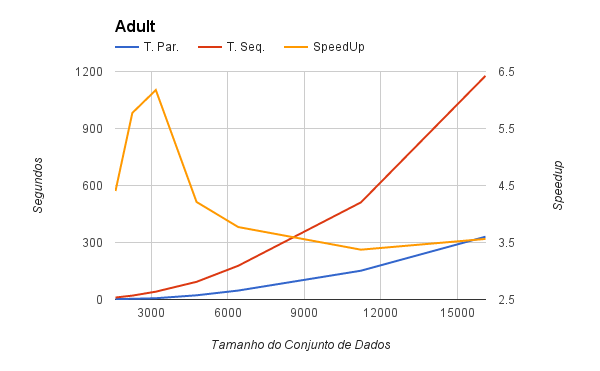
\includegraphics[width=1\textwidth]{imagens/GraficoAdult.png}
  \caption{Resultados do Conjunto de Dados \emph{Adult}}
  \label{fig:GraficoAdult}
\end{figure}

%Na Tabela \ref{tab:bestResults2w} vemos os resultados quando aumentamos o tamanho do conjunto de dados \emph{Web}.

Na Tabela \ref{tab:bestResults2w} apresentamos o tempo sequencial e paralelo conforme aumentamos os exemplos no conjunto de dados \emph{Web}. Podemos observar que a porcentagem de acertos caiu em quase 10\%. O speedup foi maior para conjuntos menores e se estabilizou por volta de $2.5$ nos conjuntos maiores que $7,366$. Podemos ver a diferença na Figura \ref{fig:GraficoAdult} que mostra um gráfico com os tempos e o speedup em relação ao tamanho do conjunto. Percebemos pela queda de porcentagem de acertos que os parâmetros que geram o melhor resultado variam com o tamanho do conjunto de dados.

%silvana: apontar motivos para a queda da precisão e do speedup

\begin{table}
    \caption{Segunda Rodada de Testes para conjunto \emph{Web}}
    \label{tab:bestResults2w}
    \small
    \centering
    \begin{tabular}{|c|c|c|c|c|c|} \hline
		Conjunto & Exemplos & T. Par. & T. Seq. & Speedup & \% Acertos\\ \hline
		\em{Web} & 2477 & 0:00:09.273 & 0:00:59.587 & 6.425860086 & 98.0617\\ \hline
		\em{Web} & 3470 & 0:00:24.333 & 0:01:56.124 & 4.772284565 & 88.5303\\ \hline
		\em{Web} & 4912 & 0:01:04.863 & 0:03:57.542 & 3.66221113 & 89.4944\\ \hline
		\em{Web} & 7366 & 0:03:36.372 & 0:08:44.351 & 2.423377332 & 89.7095\\ \hline
		\em{Web} & 9888 & 0:06:10.982 & 0:15:41.204 & 2.537061097 & 89.7956\\ \hline
		\em{Web} & 17188 & 0:19:50.535 & 0:47:21.126 & 2.38642795 & 90.3246\\ \hline
    \end{tabular}
\end{table}

\begin{figure}
  \centering
  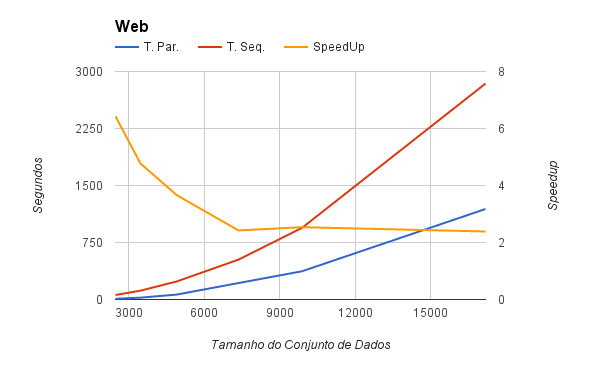
\includegraphics[width=1\textwidth]{imagens/GraficoWeb.png}
  \caption{Resultados do Conjunto de Dados \emph{Web}}
  \label{fig:GraficoWeb}
\end{figure}

Em todas os testes a versão paralela executou em menos tempo que a sequencial. O comportamento para conjuntos grandes foi similar entre os dois conjuntos, mas percebemos que tivemos uma variação anormal no speedup para o conjunto \emph{Adult}. Pelos nossos testes não conseguimos identificar porque ele cresce, depois diminui depois estabiliza.

\section{Resultados do LIBSVM}

Para efeito de comparação, medimos os resultados do LIBSVM \cite{art:LIBSVM}. Na Tabela \ref{tab:libsvmResults} apresentamos o tempo de execução e a porcentagem de acerto do LIBSVM para os conjuntos de dados que utilizamos. O LIBSVM usa os valores default: precisão de parada $p=0.001$ para interromper a execução, gama $g=(1/nAtributos)$ e controle de margem $c=1$. As medidas são de validação cruzada com 10 partições.
\begin{table}
    \caption{Resultados do LIBSVM}
    \label{tab:libsvmResults}
    \small
    \centering
    \begin{tabular}{|c|c|c|c|} \hline
        Conjunto & Exemplos & Tempo & \% Acerto \\ \hline
        \em{Adult} & 1605 & 00:00:01:52 & 83.0530 \\ \hline
        \em{Adult} & 2265 &  00:00:02:57 & 81.8102 \\ \hline
        \em{Adult} & 3185 &  00:00:04:41 & 83.1397 \\ \hline
        \em{Adult} & 4781 & 00:00:09:38 & 83.4553 \\ \hline
        \em{Adult} & 6414 & 00:00:16:45 & 83.8011 \\ \hline
        \em{Adult} & 11220 & 00:00:51:58 & 83.8146 \\ \hline
        \em{Adult} & 16100 & 00:01:49:48 & 84.0497 \\ \hline
        \em{Web} & 2477 & 00:00:00:89 & 97.0933 \\ \hline
        \em{Web} & 3470 & 00:00:01:40 & 96.9164 \\ \hline
        \em{Web} & 4912 & 00:00:02:27 & 97.0888 \\ \hline
        \em{Web} & 7366 & 00:00:04:33 & 97.0676 \\ \hline
        \em{Web} & 9888 & 00:00:07:13 & 97.1582 \\ \hline
        \em{Web} & 17188 & 00:00:20:39 & 97.0386 \\ \hline
    \end{tabular}
\end{table}

Quanto à porcentagem de acertos, nossos resultados ficaram bem próximos do LIBSVM com o conjunto {\em Adult}, de 1\% a 2\% de diferença. Com o conjunto {\em Web} o resultado foi 1\% melhor no primeiro caso, mas de 1\% a 8\% pior para os seguintes, isso nos mostra que o LIBSVM tem um resultado mais consistente, enquanto a nossa implementação depende mais da escolha certa de parâmetros.

Quanto ao tempo de execução é complicado comparar os tempos da nossa implementação com a do LIBSVM que usa um algoritmo muito mais sofisticado e complexo, logo, é compreensível que o tempo de execução de nosso programa tenha sido inferior.